\documentclass{article}
\usepackage{tikz}
\usepackage{siunitx}
\usepackage{forest}
\usepackage{cleveref}
\usetikzlibrary{arrows.meta,shapes,positioning}
\usepackage{../themeKonstanz}
\usepackage{pgfplots}

\usetikzlibrary{arrows,shapes,positioning}
\usetikzlibrary{decorations.markings}

\tikzset{fontscale/.style = {font=\relsize{#1}}
    }
\usetikzlibrary{arrows.meta,shapes,positioning}
\tikzset{MyArrow/.style={single arrow, draw, minimum width=8mm, minimum height=5mm,
                         inner sep=0mm, single arrow head extend=1mm}}

\begin{document}
\begin{figure}
    \centering
    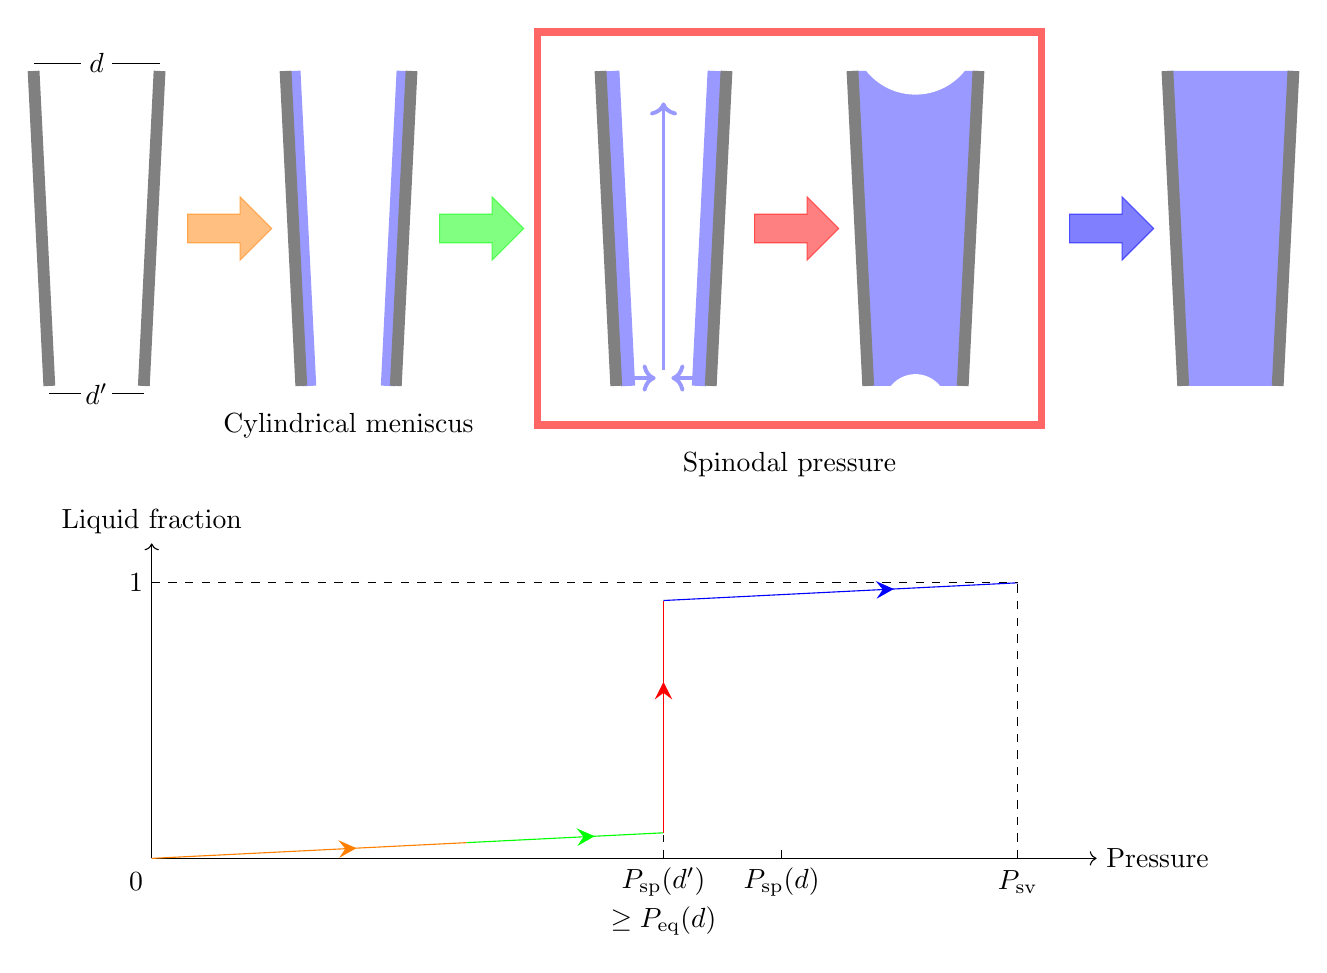
\begin{tikzpicture}[pore/.style = {line width = 0.15cm, color = gray},
                        film/.style = {line width = 0.18cm, color = blue!40},
                        thick_film/.style = {line width = 0.3cm, color = blue!40},
                        graph_label/.style={color = gray, line width = 0.05cm},
                        pore_collapse/.style = {color = blue!50, line width = 0.07cm, ->},
                        MyArrow/.style={single arrow, draw, minimum width=8mm, minimum height=5mm,
                        inner sep=0mm, single arrow head extend=1mm}]
        \pgfdeclarelayer{bg}    % declare background layer
        \pgfdeclarelayer{bbg}    % declare backbackground layer
        \pgfsetlayers{bbg,bg,main}  % set the order of the layers (main is the standard layer)
        \tikzstyle arrowstyle=[scale=2]
        \tikzstyle directed=[postaction={decorate,decoration={markings,
            mark=at position .65 with {\arrow[arrowstyle]{stealth}}}}]
        \begin{scope}
            \foreach \Xcoor in {0, 3.2, 7.2, 10.4, 14.4}
            \draw[pore] (\Xcoor + 0.2,0) -- (\Xcoor,4);
            \foreach \Xcoor in {1.6, 4.8, 8.8, 12, 16}
            \draw[pore] (\Xcoor - 0.2,0) -- (\Xcoor,4);
            \draw (0.6,4.1) -- (0,4.1); 
            \draw (1,4.1) -- (1.6,4.1); 
            \node at (0.8,4.1) {$d$};
            \draw (0.6,-0.1) -- (0.2,-0.1); 
            \draw (1,-0.1) -- (1.4,-0.1); 
            \node at (0.8,-0.1) {$d'$};
            \node[draw = orange!70, fill = orange!50, MyArrow] at (2.4, 2) {\phantom{arrow}};
            \node[draw = green!70, fill = green!50, MyArrow] at (5.6, 2) {\phantom{arrow}};
            \node[draw = red!70, fill = red!50, MyArrow] at (9.6, 2) {\phantom{arrow}};
            \node[draw = blue!70, fill = blue!50, MyArrow] at (13.6, 2) {\phantom{arrow}};
            %
            \draw[color = red!60, line width = 0.1cm] (6.4,-0.5) -- (12.8,-0.5) -- (12.8,4.5) -- (6.4,4.5) -- cycle;
            \node at (9.6,-1) {Spinodal pressure};
            \node at (4,-0.5) {Cylindrical meniscus};
            \begin{pgfonlayer}{bg}    % select the background layer
                %filmed pore
                \draw[film] (3.5,0) -- (3.3,4);
                \draw[film] (4.5,0) -- (4.7,4);
                %filmed pore
                \draw[film] (7.55,0) -- (7.35,4);
                \draw[film] (8.45,0) -- (8.65,4);
                %full pore with menisci
                \fill[blue!40] (10.6,0) -- (10.4,4)  -- (12,4) -- (11.8,0) -- cycle ;
                \draw[color = blue!40, ->, line width = 0.5mm] (7.4,0.1) -- (7.9,0.1);
                \draw[color = blue!40, ->, line width = 0.5mm] (8.6,0.1) -- (8.1,0.1);
                \draw[color = blue!40, ->, line width = 0.5mm] (8,0.2) -- (8,3.6);
                \path [draw = none, fill = white](10.4,4.5) arc[start angle = -180, end angle = 0, radius=0.8];
                \path [draw = none, fill = white](10.8,-0.25) arc[start angle = 180, end angle = 0, radius=0.4];
                %full pore
                \fill[blue!40] (14.6,0) -- (14.4,4)  -- (16,4) -- (15.8,0) -- cycle ;
            \end{pgfonlayer}
        \end{scope}
        \begin{scope}[xshift = 1.5cm, yshift=-6cm]
            \draw[->] (0,0) -- (0,4) node[anchor=south] {Liquid fraction};
            \draw[->] (0,0) -- (12,0) node[anchor=west] {Pressure};
            %yellow
            \draw[color = orange, directed] (0,0) -- (4,0.2);
            %green
            \draw[color = green, directed] (4,0.2) -- (6.5,0.325);
            %red
            \draw[color = red, directed] (6.5,0.325) -- (6.5,3.275);
            %blue
            \draw[color = blue, directed] (6.5,3.275) -- (11,3.5);
            %DASHED
            \draw[dashed] (0,3.5) -- (11,3.5);  %1
            \draw[dashed] (11,0) -- (11,3.5);  %psat
            \draw[dashed] (6.5,0) -- (6.5,0.3);  %psp
            \draw[dashed] (8,0) -- (8,0.15);  %peq
            %labels
            \node at (-0.2,-0.3) {$0$};
            \node at (-0.2,3.5) {$1$};
            \node at (11,-0.3) {$P_\mathrm{sv}$};
            \node at (6.5,-0.3) {$P_\mathrm{sp}(d')$};
            \node at (6.5,-0.8) {$\ge P_\mathrm{eq}(d)$};
            \node at (8,-0.3) {$P_\mathrm{sp}(d)$};
        \end{scope}
    \end{tikzpicture}
    \caption{Absorption isotherm of a funnelled cylindrical pore. Below, the processes inside the pore are illustrated. The colors of the broad arrow's colors correspond to the pressure ranges of the isotherm in the same color. Significant is the absorption at spinodal pressure of the smallest occuring diameter. Even though only a liquid bridge at the smallest part of the pore is created, the pore fills completely as the equilibrium pressure of any part of the pore is smaller than the spinodal pressure.}
    \label{fig:perf-cyl-pores-cond}
\end{figure}
\end{document}

%Condensation process inside a funnelled cylindrical pore. When increasing vapor pressure a film of increasing thickness forms on the inside of the pore. Upon reaching spinodal pressure of the pore radius $r'$, the film collapsed to the inside. As of now, the pore is closed on the small end and moreover equilibrium pressure even of the larger raius $r$ is smaller than $P_\mathrm{sp}(r')$, the pore fills starting at the liquid bridge leaving only a meniscus at either end. The latter widens when further increasing the pressure and fully disappears at saturated vapor pressure. The graph shows the liquid fraction condensed inside the pore depending on the current vapor pressure. The slopes before and after the condensation at spinodal pressure $P_\mathrm{sp}(r')$ imply the thickening of the film and the relaxation of the menisci.